\section{中間ポジション(2/2)}

\begin{center}
\begin{tabular}{|lcl|}
\hline
この章の基礎練習 & : & 1. 開放弦の練習 2. 「\ref{5th_scale}」「\ref{2nd-3rd_scale}」の音階練習 3. 「どろぼうかささぎ」 4. モーツァルト\\
この章の修了課題 & : & 1. 「\ref{5th-6th_scale}」の音階練習を正しい音程で暗譜して演奏できる\\
               &   & 2. ドヴォルザークを正しい音程で暗譜して演奏できる\\
\hline
\end{tabular}
\end{center}

\begin{flushleft}
\begin{minipage}{280pt}
\subsection{第V・第VIの中間ポジションの位置}
\ \ 第Vポジションの半音上に位置します。第IV、第Vポジションがそれぞ
れ隣の弦の第I、第IIポジションに対応していたように、第V・第VIの中間ポジ
ションで取れる音は、細い方の隣の弦の第II・第IIIの中間ポジションの音に対応し
ています。\underline{\bf 4の指を用いるのはこのポジションまでです。}次
の第6ポジションからは今まで使わなかった3の指を代わりに用います。
\subsection{第V・第VIの中間ポジションで取れる音}
\begin{music}
\nostartrule
\parindent 0pt
\setclef1{\bass}  
\startpiece
\notes\enotes
\Notes\zchar{18}{G線}\zchar{14}{\bf 1}\wh{e}\zchar{15}{\bf 2}\wh{f}\zchar{15}{\bf 4}\wh{^f}\enotes
\doublebar
\Notes\zchar{14}{\bf 1}\wh{e}\zchar{15}{\bf 2}\wh{f}\zchar{16}{\bf 4}\wh{_g}\enotes
\doublebar
\Notes\zchar{18}{D線}\zchar{11}{\bf 1}\wh{b}\zchar{12}{\bf 2}\wh{c}\zchar{12}{\bf 4}\wh{^c}\enotes
\doublebar
\Notes\zchar{11}{\bf 1}\wh{b}\zchar{12}{\bf 2}\wh{c}\zchar{13}{\bf 4}\wh{_d}\enotes
\setdoublebar
\endpiece
\startpiece
\notes\enotes
\Notes\zchar{14}{A線}\zchar{9}{\bf 1}\wh{'^F}\zchar{9}{\bf 2}\wh{G}\zchar{9}{\bf 4}\wh{^G}\enotes
\doublebar
\Notes\zchar{10}{\bf 1}\wh{'_G}\zchar{10}{\bf 2}\wh{=G}\zchar{10}{\bf 4}\wh{!_a}\enotes
\doublebar
\Notes\zchar{14}{E線}\zchar{9}{\bf 1}\wh{'^C}\zchar{9}{\bf 2}\wh{D}\zchar{9}{\bf 4}\wh{^D}\enotes
\doublebar
\Notes\zchar{9}{\bf 1}\wh{'_D}\zchar{9}{\bf 2}\wh{=D}\zchar{9}{\bf 4}\wh{_E}\enotes
\setdoublebar
\endpiece
\end{music}
\end{minipage}
\hfill
\begin{minipage}{140pt}
\addtocounter{figure}{1}
\begin{center}
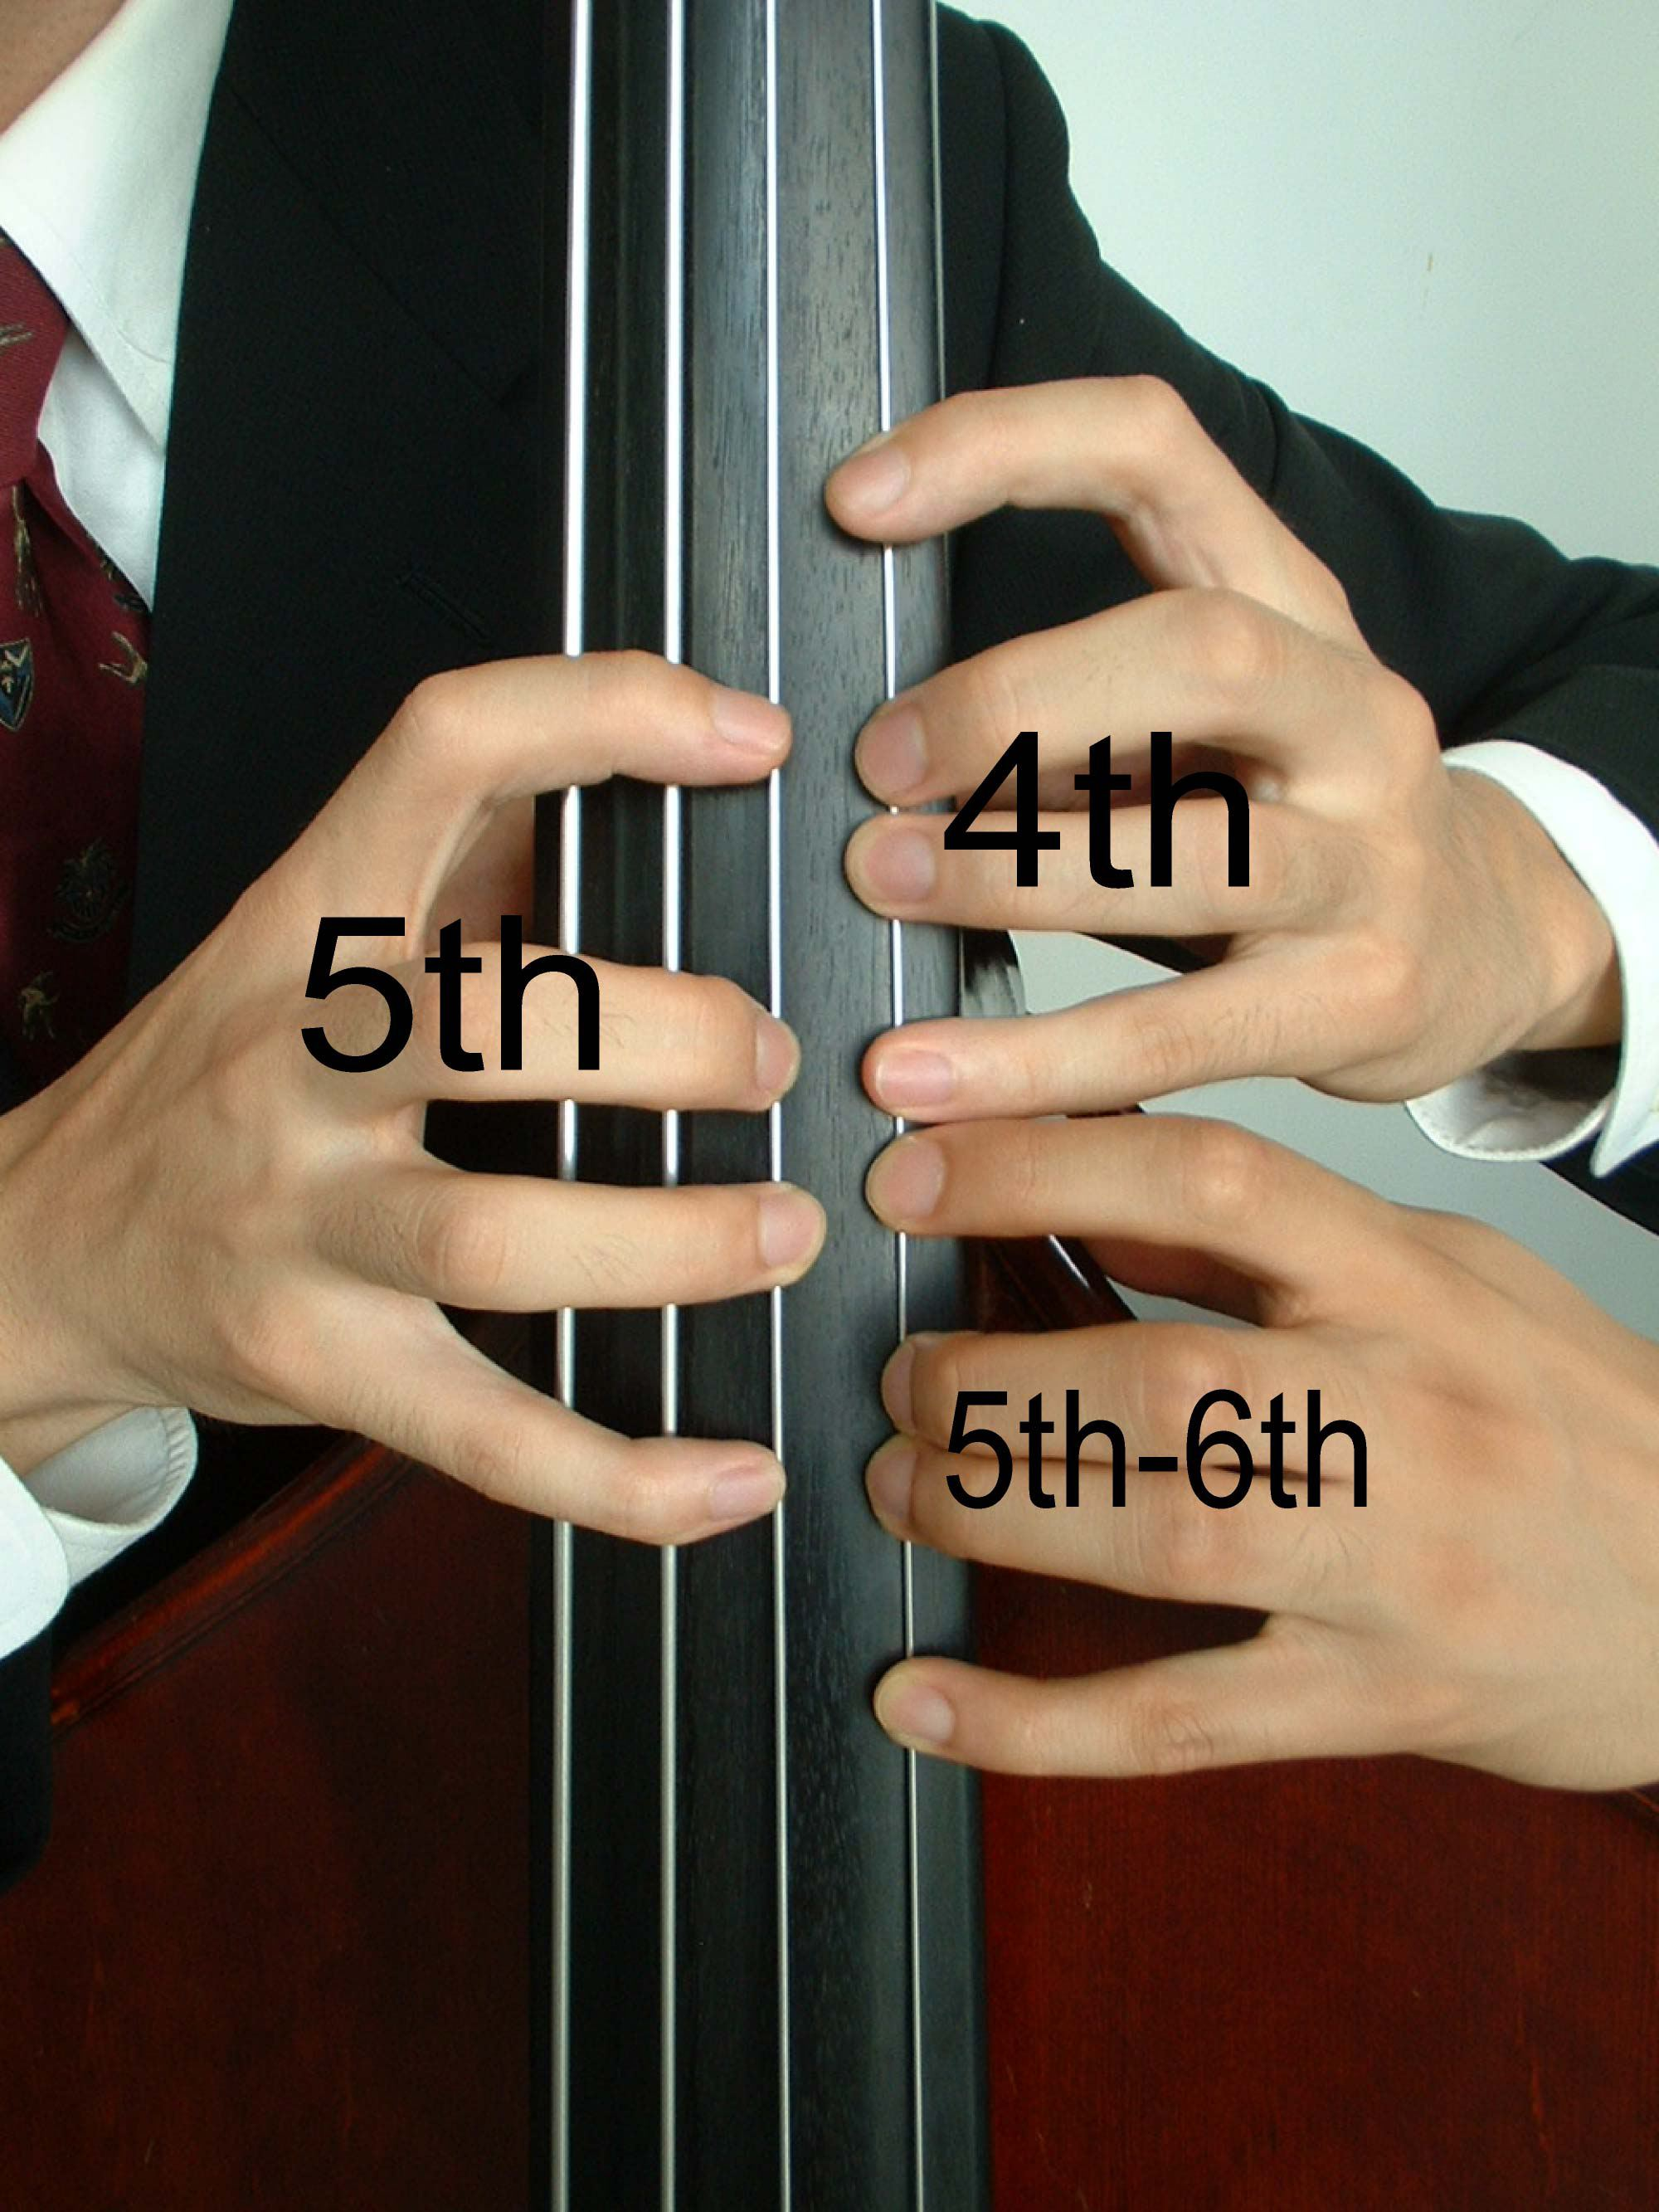
\includegraphics[width=4.5cm]{Pics/newphoto/5th-6th.epsi}\\
{\flushleft\small 図\thefigure : 第V・第VIの中間ポジション(図の上から4th、5th、5th-6th)\\}
\end{center}
\end{minipage}
\end{flushleft}

\subsection{音階練習 \label{5th-6th_scale}}
\begin{music}
\nostartrule
\parindent 0pt
\setclef1{\bass}  
\generalsignature{-6}    
\startpiece
\notes\zchar{14}{変ト長調(Ges-dur)音階}\enotes
\Notes\zchar{-4}{I}\zchar{8}{\bf 1}\qu{G}\enotes
\notes\ibu{0}{'A}{3}\islurd{0}{A}\qb{0}{A}\tbu{0}\tslur{0}{B}\loffset{0.8}{\zchar{-5}{\small half}}\zchar{9}{\bf 1}\qb{0}{B}\enotes
\notes\ibl{0}{'C}{3}\zchar{-7}{I}\zchar{8}{\bf 1}\qb{0}{C}\qb{0}{D}\loffset{1}{\zchar{-7}{\small half}}\zchar{8}{\bf 1}\qb{0}{E}\tbl{0}\zchar{-5}{I}\zchar{8}{\bf 2}\qb{0}{F}\enotes
\bar
\Notes\ql{'G}\enotes
\notes\ibl{0}{a}{3}\isluru{0}{a}\loffset{1}{\zchar{-4}{\small half}}\zchar{11}{\bf 1}\qb{0}{a}\tbl{0}\tslur{0}{b}\roffset{0.25}{\zchar{-4}{I}}\zchar{12}{\bf 2}\qb{0}{b}\enotes
\notes\ibl{0}{c}{3}\qb{0}{c}\loffset{0.7}{\zchar{-4}{\small [}}\zchar{-3}{\small III}\zchar{-6}{\small IV}\zchar{13}{\bf 1}\qb{0}{d}\qb{0}{e}\tbl{0}\loffset{0.7}{\zchar{-4}{\small [}}\roffset{0.3}{\zchar{-3}{\small V}}\zchar{-6}{\small VI}\zchar{15}{\bf 2}\qb{0}{f}\enotes
\bar
\Notes\zchar{16}{\bf 4}\ql{g}\enotes
\notes\ibl{0}{f}{-2}\isluru{0}{f}\qb{0}{f}\tbl{0}\tslur{0}{e}\loffset{0.7}{\zchar{-4}{\small [}}\zchar{-3}{\small III}\zchar{-6}{\small IV}\zchar{15}{\bf 4}\qb{0}{e}\enotes
\notes\ibl{0}{d}{-3}\qb{0}{d}\zchar{-4}{II}\zchar{12}{\bf 4}\qb{0}{c}\qb{0}{b}\tbl{0}\loffset{0.3}{\zchar{-4}{\small half}}\zchar{10}{\bf 1}\qb{0}{a}\enotes
\bar
\notes\ibl{0}{'G}{-3}\zchar{-4}{I}\zchar{10}{\bf 4}\qb{0}{G}\qb{0}{F}\loffset{1}{\zchar{-6}{\small half}}\zchar{8}{\bf 1}\qb{0}{E}\tbl{0}\zchar{-5}{I}\zchar{8}{\bf 4}\qb{0}{D}\enotes
\notes\ibu{0}{'C}{-3}\qb{0}{C}\loffset{1}{\zchar{-6}{\small half}}\zchar{-3}{\bf 1}\qb{0}{B}\roffset{0.4}{\zchar{-8}{I}}\zchar{-4}{\bf 4}\qb{0}{A}\tbu{0}\qb{0}{!G}\enotes
\endpiece

\generalsignature{3}    
\startpiece
\notes\zchar{14}{嬰ヘ短調(fis-moll)音階}\enotes
\Notes\zchar{-6}{I}\zchar{8}{\bf 1}\qu{F}\enotes
\notes\ibu{0}{G}{3}\islurd{0}{G}\qb{0}{G}\tbu{0}\tslur{0}{'A}\qb{0}{A}\enotes
\notes\ibl{0}{'B}{3}\qb{0}{B}\qb{0}{C}\loffset{1}{\zchar{-8}{half}}\zchar{8}{\bf 1}\qb{0}{^D}\tbl{0}\zchar{-6}{I}\zchar{8}{\bf 2}\qb{0}{^E}\enotes
\bar
\Notes\ql{'F}\enotes
\notes\ibl{0}{'G}{3}\isluru{0}{G}\loffset{1.4}{\zchar{-4}{\small half}}\zchar{10}{\bf 1}\qb{0}{G}\tbl{0}\tslur{0}{!a}\zchar{-4}{I}\zchar{11}{\bf 1}\qb{0}{a}\enotes
\notes\ibl{0}{b}{3}\qb{0}{b}\loffset{0.7}{\zchar{-4}{\small [}}\zchar{-3}{\small III}\zchar{-6}{\small IV}\zchar{12}{\bf 1}\qb{0}{c}\qb{0}{^d}\tbl{0}\loffset{0.7}{\zchar{-4}{\small [}}\roffset{0.3}{\zchar{-3}{\small V}}\zchar{-6}{\small VI}\zchar{14}{\bf 2}\qb{0}{^e}\enotes
\bar
\Notes\zchar{15}{\bf 4}\ql{f}\enotes
\notes\ibl{0}{e}{-2}\isluru{0}{e}\qb{0}{=e}\tbl{0}\tslur{0}{d}\zchar{-4}{III}\zchar{14}{\bf 4}\qb{0}{=d}\enotes
\notes\ibl{0}{c}{-3}\qb{0}{c}\zchar{-4}{I}\zchar{12}{\bf 4}\qb{0}{b}\qb{0}{a}\tbl{0}\loffset{0.7}{\zchar{-4}{\small [}}\roffset{0.3}{\zchar{-3}{\small II}}\zchar{-6}{\small III}\zchar{10}{\bf 4}\qb{0}{'G}\enotes
\bar
\notes\ibl{0}{'F}{-3}\qb{0}{F}\loffset{0.4}{\zchar{-6}{\small half}}\zchar{8}{\bf 2}\qb{0}{E}\qb{0}{D}\tbl{0}\zchar{-6}{I}\zchar{8}{\bf 4}\qb{0}{C}\enotes
\notes\ibu{0}{'B}{-3}\qb{0}{B}\qb{0}{A}\qb{0}{!G}\tbu{0}\qb{0}{F}\enotes
\endpiece
\end{music}

\clearpage

\begin{flushleft}
\begin{minipage}{200pt}
\subsection{ピッツィカート(伊 pizzicato)}
\ \ \ \ 譜面上にpizz.と書いてあったら、それ以降の音符は右手の指で弦を
はじいて演奏します。これをピッツィカート奏法と呼びます。ピッツィカート
はarcoと書かれている地点まで続きます。arco以降は元通り弓で演奏します。
強いピッツィカート音を出したいときは人さし指と中指の2本で、小さい音が
欲しいときは人さし指1本ではじきます。
\end{minipage}
\hfill
\begin{minipage}{60pt}
\begin{center}
\addtocounter{figure}{1}
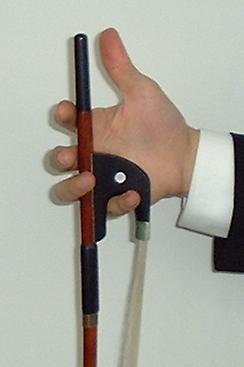
\includegraphics[height=4.5cm]{Pics/Pizz/pizz_1.epsi}\\
図\thefigure \\
\end{center}
\end{minipage}
\hfill
\begin{minipage}{90pt}
\begin{center}
\addtocounter{figure}{1}
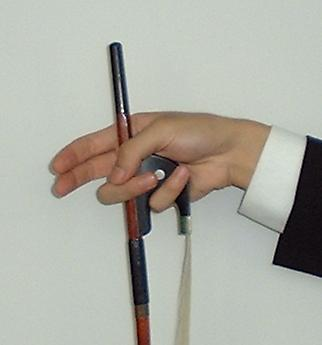
\includegraphics[height=4.5cm]{Pics/Pizz/pizz_2.epsi}\\
図\thefigure \\
\end{center}
\end{minipage}
\end{flushleft}

\begin{minipage}{100pt}
\begin{center}
\addtocounter{figure}{1}
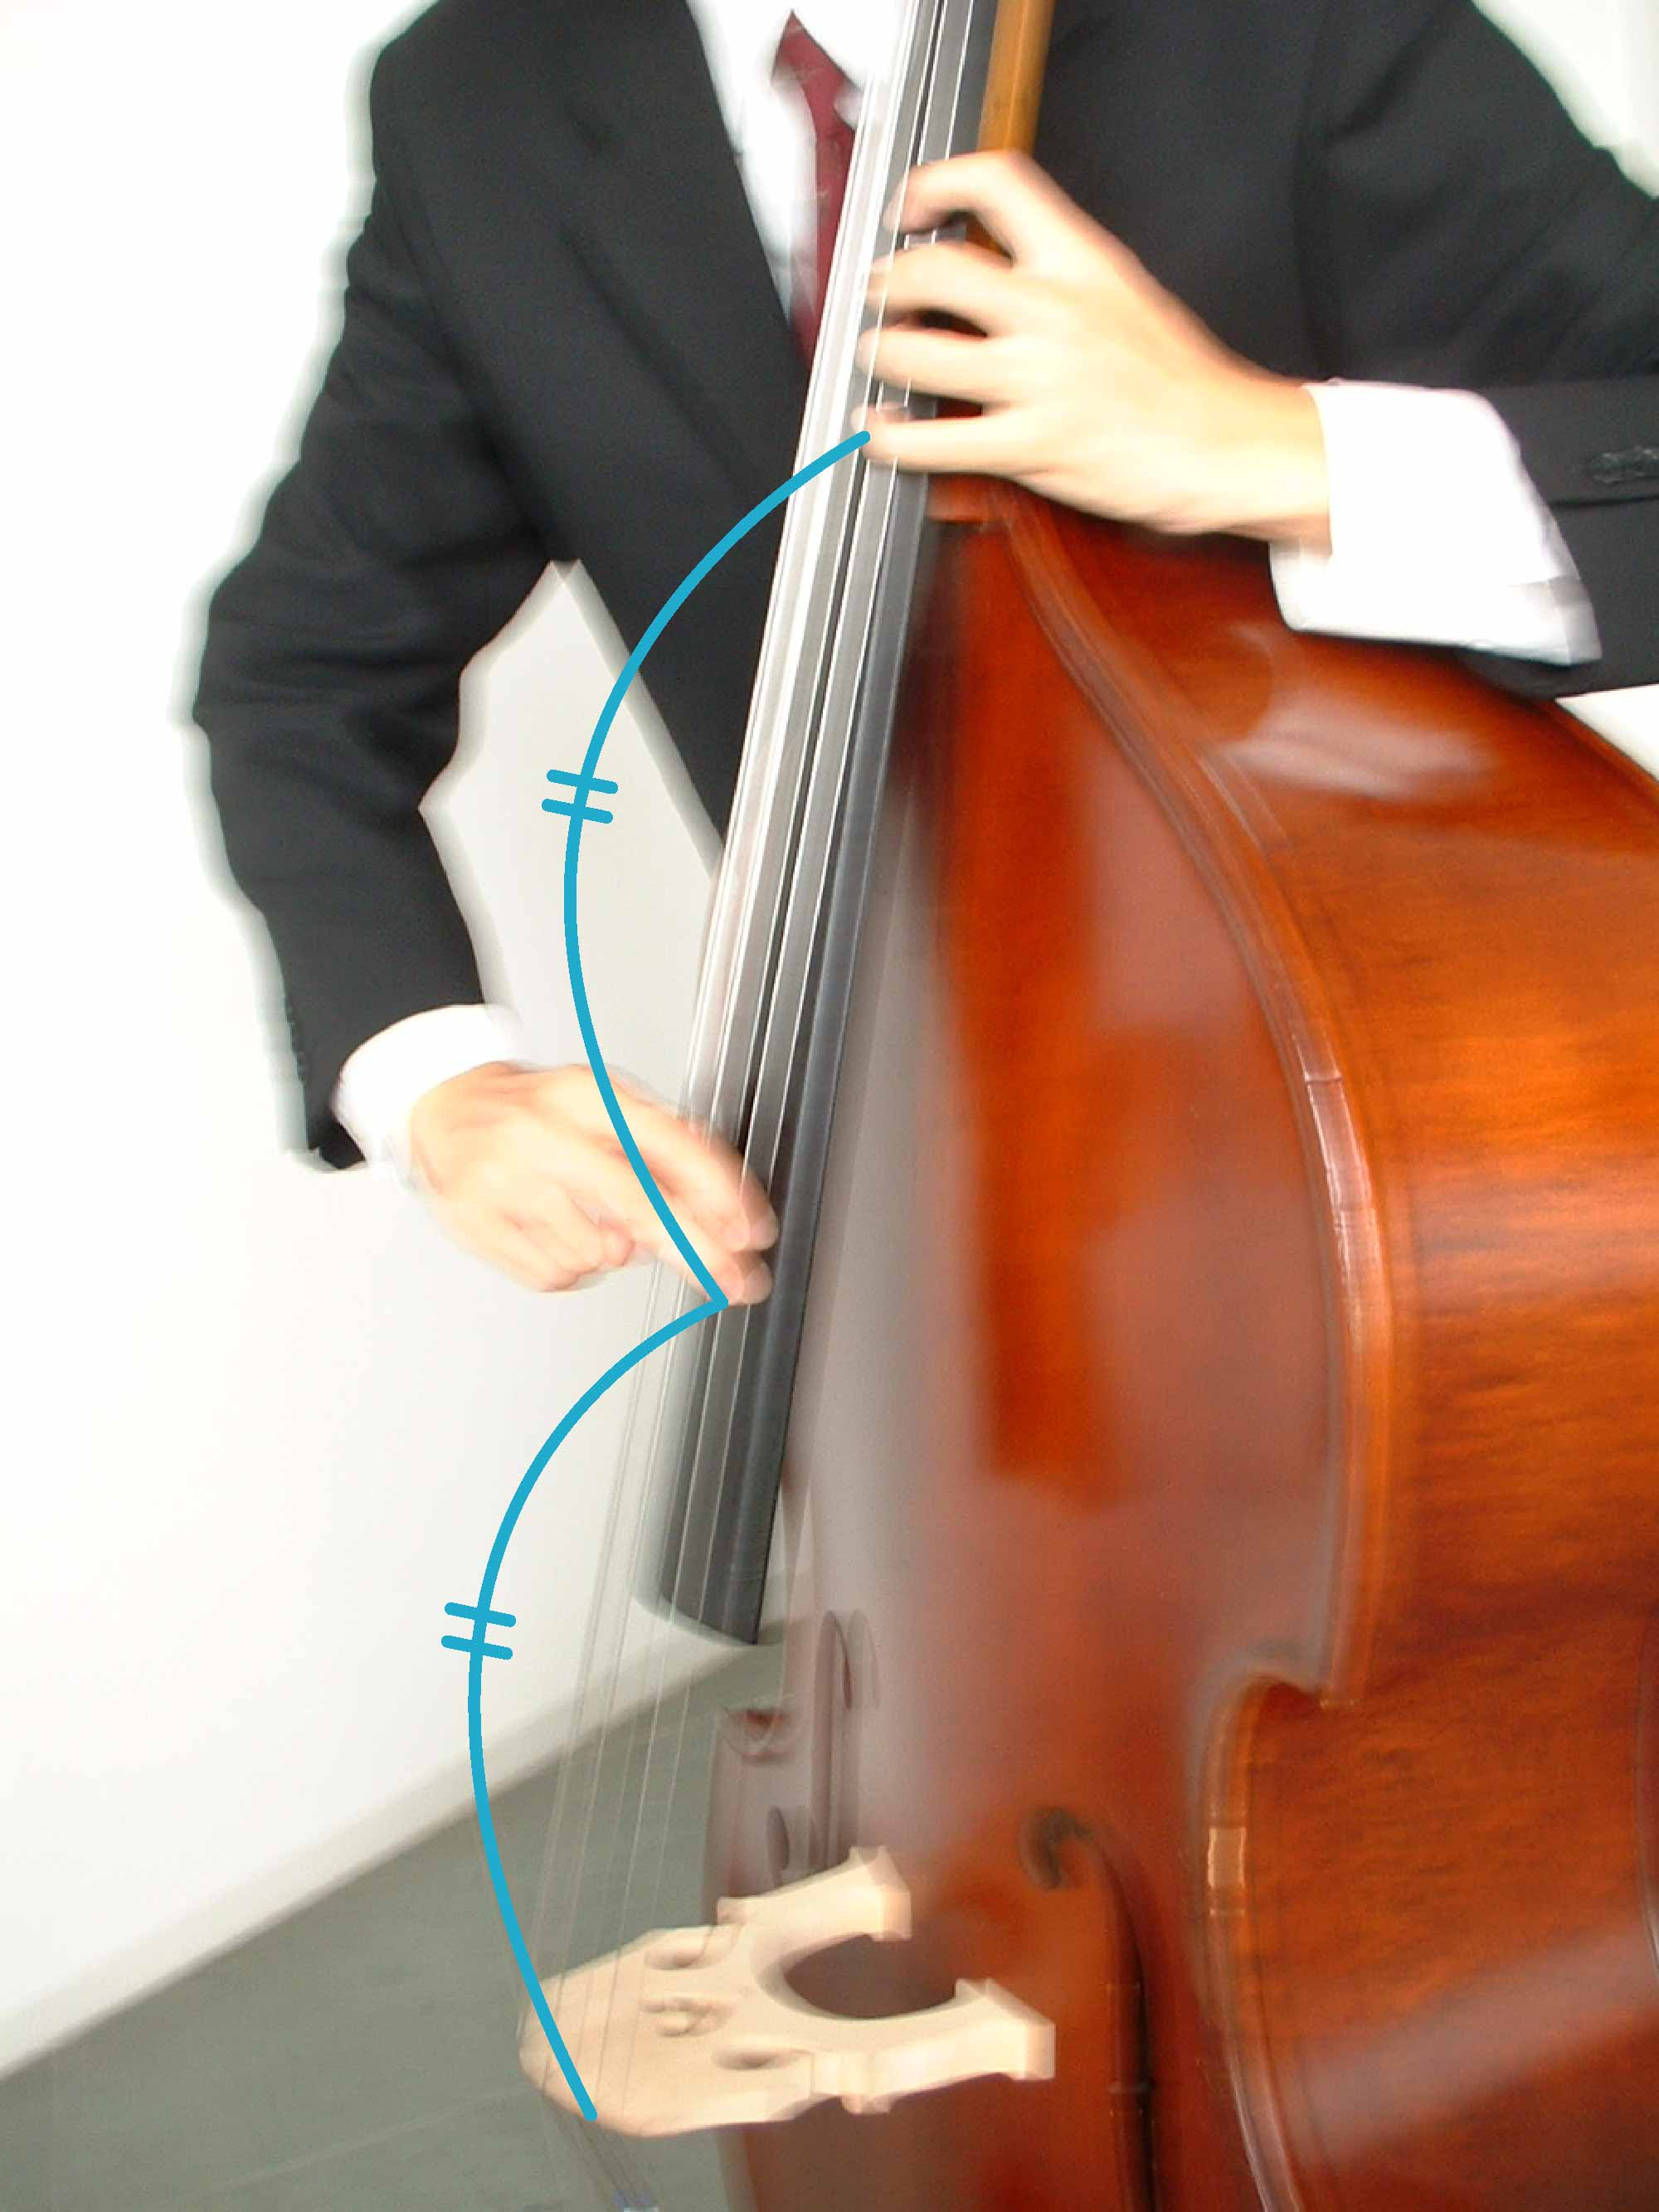
\includegraphics[height=4.5cm]{Pics/photo0830/pizz_point.epsi}\\
図\thefigure \\
\end{center}
\end{minipage}
\hfill
\begin{minipage}{100pt}
\begin{center}
\addtocounter{figure}{1}
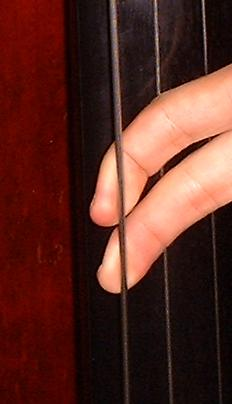
\includegraphics[height=4.5cm]{Pics/Pizz/pizz_3.epsi}\\
図\thefigure \\
\end{center}
\end{minipage}
\hfill
\begin{minipage}{220pt}
\begin{center}
\addtocounter{figure}{1}
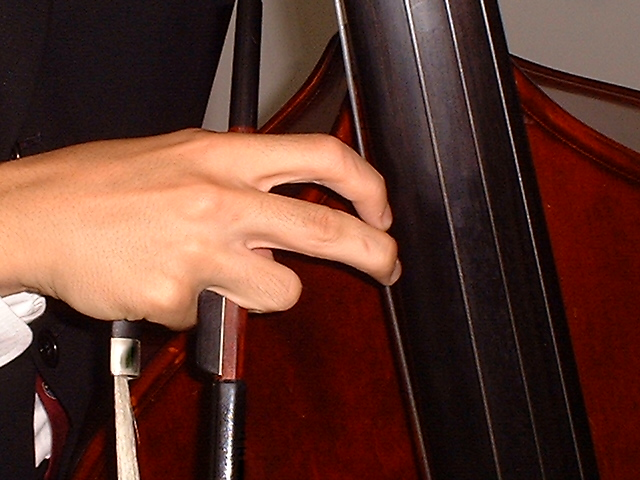
\includegraphics[height=4.5cm]{Pics/Pizz/pizz_4.epsi}\\
図\thefigure \\
\end{center}
\end{minipage}

\begin{enumerate}
\item まず小指に弓を引っ掛けます(\addtocounter{figure}{-4}図\thefigure )。
\item 弓を握ります(\addtocounter{figure}{1}図\thefigure )。
\item 左手で押さえた地点から駒までの中間点に右手の指を持って行きます(\addtocounter{figure}{1}図\thefigure )。
\item 指を弦に押し当て、指先に「肉溜まり」をつくります(\addtocounter{figure}{1}図\thefigure )。
\item 弦を横方向に引っ張ります(\addtocounter{figure}{1}図\thefigure )。
\item 弦を放し、エネルギーを一気に開放します。弦を指板に当てて雑音を出さないように注意しましょう。
\end{enumerate}

\subsection{中間ポジションで弾ける名曲}
%シャープ系は白鳥湖のワルツ、未完成
\documentclass{jarticle}
\usepackage{musixdoc}
\startmuflex\makeindex

\begin{document}

\subsubsection*{�ɥ����륶����: �������9�� ��ûĴ �ֿ��������� ��2�ھϤ��}

\begin{music}
\nostartrule
\setclef1{\bass}
\generalsignature{4}    
\generalmeter{\meterC}
\parindent 0pt
\startbarno=54
\def\writebarno{\tenrm\the\barno\barnoadd}
\def\raisebarno{2\internote}
\def\shiftbarno{0.1\Interligne}
\systemnumbers
\startpiece\bigaccid
\notes\zchar{18}{\bf Poco meno mosso (Largo $\rightarrow$ Un poco pi\`u mosso $\rightarrow$)}\zchar{14}{pizz.}\enotes
\Notes\ibl{0}{'C}{0}\zchar{-10}{\pp}\zchar{-7}{I}\zchar{9}{\bf 4}\qb{0}{CE}\loffset{0.7}{\zchar{-8}{\small [}}\roffset{0.3}{\zchar{-7}{\small II}}\zchar{-10}{\small III}\zchar{9}{\bf 4}\qb{0}{G}\tbl{0}\qb{0}{C}\enotes
\Notes\ibl{0}{'F}{-3}\zchar{-5}{I}\zchar{9}{\bf 4}\qb{0}{F!a}\loffset{0.7}{\zchar{-8}{\small [}}\roffset{0.3}{\zchar{-7}{\small II}}\zchar{-10}{\small III}\zchar{9}{\bf 4}\qb{0}{'G}\tbl{0}\qb{0}{C}\enotes
\bar
\Notes\ibl{0}{'F}{5}\qb{0}{F}\zchar{-4}{III}\zchar{9}{\bf 4}\qb{0}{!a=d}\tbl{0}\loffset{0.7}{\zchar{-5}{\small [}}\roffset{0.3}{\zchar{-4}{\small V}}\zchar{-7}{\small VI}\zchar{14}{\bf 1}\qb{0}{e}\enotes
\Notes\ibl{0}{f}{-3}\zchar{15}{\bf 4}\qb{0}{f}\zchar{-4}{III}\zchar{13}{\bf 4}\qb{0}{dc}\tbl{0}\qb{0}{^b}\enotes
\bar
\Notes\ibl{0}{c}{-2}\qb{0}{c}\zchar{-4}{V}\zchar{13}{\bf 1}\qb{0}{^d}\qb{0}{e}\tbl{0}\qb{0}{^a}\enotes
\Notes\ibl{0}{'G}{0}\qb{0}{!^b}\zchar{-4}{III}\zchar{9}{\bf 2}\qb{0}{'G!c}\tbl{0}\qb{0}{=a}\enotes
\bar
\Notes\ibl{0}{'F}{0}\loffset{0.7}{\zchar{-6}{\small [}}\roffset{0.3}{\zchar{-5}{\small II}}\zchar{-8}{\small III}\zchar{9}{\bf 1}\qb{0}{FG}\zchar{-5}{I}\zchar{10}{\bf 1}\qb{0}{!a}\tbl{0}\qb{0}{'F}\enotes
\Notes\ibl{0}{'D}{3}\loffset{0.7}{\zchar{-8}{\small [}}\roffset{0.3}{\zchar{-7}{\small II}}\zchar{-10}{\small III}\zchar{9}{\bf 4}\qb{0}{D}\tbl{0}\qb{0}{F}\enotes
\Notes\ibu{0}{'G}{-8}\qb{0}{G}\tbu{0}\qb{0}{!G}\enotes
\bar
\Notes\ibl{0}{'C}{5}\zchar{-10}{\pp}\zchar{-7}{I}\zchar{9}{\bf 4}\qb{0}{CE}\loffset{0.7}{\zchar{-6}{\small [}}\roffset{0.3}{\zchar{-5}{\small II}}\zchar{-8}{\small III}\zchar{9}{\bf 4}\qb{0}{G}\tbl{0}\qb{0}{!c}\enotes
\Notes\ibl{0}{b}{-3}\qb{0}{b}\zchar{-4}{III}\zchar{11}{\bf 4}\qb{0}{a'G}\tbl{0}\qb{0}{E}\enotes
\bar
\Notes\ibl{0}{'C}{3}\loffset{0.7}{\zchar{-8}{\small [}}\roffset{0.3}{\zchar{-7}{\small II}}\zchar{-10}{\small III}\zchar{9}{\bf 1}\qb{0}{CG}\zchar{-6}{III}\zchar{9}{\bf 4}\qb{0}{E}\tbl{0}\qb{0}{!c}\enotes
\Notes\ibl{0}{a}{2}\zchar{-4}{\it cresc.}\qb{0}{ac}\loffset{0.7}{\zchar{-5}{\small [}}\roffset{0.3}{\zchar{-4}{\small V}}\zchar{-7}{\small VI}\zchar{14}{\bf 1}\qb{0}{e}\tbl{0}\qb{0}{c}\enotes
\bar
\Notes\ibl{0}{b}{0}\zchar{-6}{\mf \decrescendo{40mm}}\qb{0}{bf}\zchar{-4}{IV}\zchar{13}{\bf 2}\qb{0}{d}\tbl{0}\qb{0}{b}\enotes
\Notes\ibl{0}{e}{-5}\qb{0}{eb}\zchar{-5}{III}\zchar{9}{\bf 2}\qb{0}{'G}\tbl{0}\qb{0}{E}\enotes
\bar
\Notes\ibl{0}{d}{-5}\zchar{-3}{\p}\qb{0}{=da}\zchar{-5}{II}\zchar{9}{\bf 2}\qb{0}{'F}\tbl{0}\qb{0}{=D}\enotes
\Notes\ibu{0}{'A}{4}\zchar{-3}{\it dim.}\qb{0}{A}\zchar{-4}{I}\zchar{11}{\bf 1}\qb{0}{BC}\tbu{0}\qb{0}{E}\enotes
\bar
\Notes\ibl{0}{'F}{0}\zchar{-11}{\pp}\loffset{0.7}{\zchar{-6}{\small [}}\roffset{0.3}{\zchar{-5}{\small II}}\zchar{-8}{\small III}\zchar{9}{\bf 1}\qb{0}{FG}\zchar{-5}{I}\zchar{11}{\bf 1}\qb{0}{!a}\tbl{0}\qb{0}{'F}\enotes
\Notes\ibu{0}{'G}{0}\loffset{0.7}{\zchar{-6}{\small [}}\roffset{0.3}{\zchar{-5}{\small II}}\zchar{-8}{\small III}\zchar{-1}{\bf 4}\qb{0}{DFG}\tbu{0}\qb{0}{!G}\enotes
\bar
\Notes\ibl{0}{'C}{4}\qb{0}{C!cb}\tbl{0}\zchar{-4}{half}\zchar{10}{\bf 2}\qb{0}{a}\enotes
\Notes\ibu{0}{'G}{-5}\qb{0}{GE}\zchar{-5}{I}\zchar{-2}{\bf 4}\qb{0}{C}\tbu{0}\qb{0}{!G}\enotes
\bar
\Notes\cu{'C}\ds\qp\hpause\enotes
\mulooseness=0
\setdoublebar\endpiece
\end{music}

\endmuflex
\end{document}

\documentclass{jarticle}
\usepackage{musixdoc}
\startmuflex\makeindex

\newcommand{\flag}[2]{\zchar{#2}{$\circ$}\zchar{#1}{\tiny +}}
\newcommand{\press}[2]{\zchar{#2}{$\circ$}\zchar{#1}{\small \|}}

\begin{document}

\subsubsection*{�ޡ��顼: �������2�� ��ûĴ ������� ��1�ھ���Ƭ}

\begin{music}
\nostartrule
\setclef1{\bass}
\generalsignature{-3}    
\generalmeter{\meterfrac44}
\parindent 0pt
\startbarno=1
\def\writebarno{\tenrm\the\barno\barnoadd}
\def\raisebarno{2\internote}
\def\shiftbarno{0.1\Interligne}
\systemnumbers
\startpiece\bigaccid
\notes\zchar{18}{\bf Allegro maestoso. Mit durchaus ernstem und feierlichem Ausdruck.}\enotes
\NOtes\hp\zchar{-4}{\it wild}\sk\enotes
\bar
\notes\zchar{8}{\ppfftwenty sf}\zchar{-4}{\fff}\enotes
\notes\usfz{c}\ibbu{0}{'C}{1}\qb{0}{C=BC}\tbbu{0}\tbu{0}\qb{0}{D}\enotes
\Notes\cl{'E}\ds\hpause\enotes
\bar 
\Notes\pause\enotes
\bar
\notes\zchar{8}{\ppfftwenty sf}\zchar{-4}{\ff}\enotes
\notes\usfz{'E}\ibbl{0}{E}{1}\qb{0}{EDE}\tbbl{0}\tbl{0}\qb{0}{F}\enotes
\Notes\cl{'G}\fermataup{G}\ds\enotes
\notes\zchar{-4}{\ff}\qs\zchar{9}{\it accel.}\ibbl{0}{'D}{3}\qb{0}{CD}\tbbl{0}\tbl{0}\qb{0}{E}\enotes
\notes\ibbl{0}{'F}{3}\qb{0}{FG=!a}\tbbl{0}\tbl{0}\qb{0}{=!b}\enotes
\bar
\Notes\zchar{-4}{\ppfftwenty sf}\ibl{0}{c}{-5}\usfz{d}\upz{c}\qb{0}{c}\enotes
\notes\raise2ex\qs\tbbl{0}\tbl{0}\upz{'G}\qb{0}{G}\enotes
\Notes\lpz{'C}\cu{C}\ds\qp\pt{E}\ds\enotes
\notes\zchar{-4}{\f}\ccl{'G}\enotes
\bar
\Notes\zchar{14}{\bf a tempo}\ibl{0}{c}{-5}\qb{0}{c}\enotes
\notes\raise2ex\qs\tbbl{0}\tbl{0}\qb{0}{'G}\enotes
\Notes\ibl{0}{c}{-5}\qb{0}{c}\enotes
\notes\raise2ex\qs\tbbl{0}\tbl{0}\qb{0}{'G}\enotes
\NOtes\ust{c}\ql{c}\enotes
\notes\ds\upz{'G}\cl{G}\enotes
\bar
\notes\ibl{0}{c}{0}\upz{c}\qb{0}{c}\upz{b}\qb{0}{=b}\tbl{0}\upz{c}\qb{0}{c}\enotes
\notes\ibl{0}{d}{-2}\upz{d}\qb{0}{d}\upz{c}\qb{0}{c}\tbl{0}\upz{b}\qb{0}{b}\enotes
\Notes\ibl{0}{c}{-5}\upz{c}\qb{0}{c}\enotes
\notes\raise2ex\qs\tbbl{0}\tbl{0}\upz{'G}\qb{0}{G}\enotes
\Notes\ibl{0}{a}{-3}\upz{a}\qb{0}{a}\enotes
\notes\raise1ex\qs\tbbl{0}\tbl{0}\upz{'F}\qb{0}{^F}\enotes
\bar
\Notes\ibl{0}{'G}{-3}\upz{G}\qb{0}{G}\enotes
\notes\zchar{-6}{\mf}\raise1ex\qs\tbbl{0}\tbl{0}\upz{'E}\qb{0}{E}\enotes
\Notes\ibl{0}{'G}{-3}\upz{G}\qb{0}{G}\enotes
\notes\raise1ex\qs\tbbl{0}\tbl{0}\upz{'E}\qb{0}{E}\enotes
\Notes\ibl{0}{'G}{-3}\upz{G}\qb{0}{G}\enotes
\notes\raise1ex\qs\tbbl{0}\tbl{0}\upz{'E}\qb{0}{E}\enotes
\qspace
\notes\ibbl{0}{'F}{-1}\upz{F}\qb{0}{=F}\upz{E}\qb{0}{E}\upz{D}\qb{0}{D}\tbbl{0}\tbl{0}\upz{E}\qb{0}{E}\enotes
\bar
\Notes\ibl{0}{'G}{-3}\upz{G}\qb{0}{G}\enotes
\notes\raise1ex\qs\tbbl{0}\tbl{0}\upz{'E}\qb{0}{E}\enotes
\Notes\ibl{0}{'G}{-3}\upz{G}\qb{0}{G}\enotes
\notes\raise1ex\qs\tbbl{0}\tbl{0}\upz{'E}\qb{0}{E}\enotes
\Notes\ibl{0}{'G}{-3}\upz{G}\qb{0}{G}\enotes
\notes\raise1ex\qs\tbbl{0}\tbl{0}\upz{'E}\qb{0}{E}\enotes
\qspace
\notes\ibbl{0}{a}{-3}\upz{a}\qb{0}{a}\upz{'G}\qb{0}{G}\upz{F}\qb{0}{F}\tbbl{0}\tbl{0}\upz{E}\qb{0}{E}\enotes
\bar
\Notes\ibl{0}{'G}{-5}\zchar{-5}{\ff}\upz{G}\qb{0}{G}\enotes
\notes\raise1ex\qs\tbbl{0}\tbl{0}\upz{'D}\qb{0}{D}\enotes
\notes\lpz{G}\cu{G}\ds\enotes
\notes\xtuplet3{c}\ds\ibl{0}{'F}{3}\upz{F}\qb{0}{F}\tbl{0}\upz{G}\qb{0}{G}\enotes
\notes\xtuplet3{d}\ibl{0}{'F}{0}\upz{!a}\qb{0}{!a}\upz{'F}\qb{0}{F}\tbl{0}\upz{!d}\qb{0}{d}\enotes
\bar
\Notes\ibl{0}{'G}{-5}\zchar{-5}{\ff}\upz{G}\qb{0}{G}\enotes
\notes\raise1ex\qs\tbbl{0}\tbl{0}\upz{'D}\qb{0}{D}\enotes
\notes\lpz{G}\cu{G}\ds\enotes
\notes\xtuplet3{c}\ds\ibl{0}{'F}{3}\upz{F}\qb{0}{F}\tbl{0}\upz{G}\qb{0}{G}\enotes
\notes\xtuplet3{d}\ibl{0}{'F}{0}\zchar{-5}{\f}\upz{!a}\qb{0}{a}\upz{'F}\qb{0}{F}\tbl{0}\upz{!d}\qb{0}{d}\enotes
\bar
\notes\zchar{-5}{\p \it subito}\xtuplet3{b}\ibl{0}{'E}{0}\qb{0}{GE}\tbl{0}\qb{0}{!c}\enotes
\notes\xtuplet3{b}\ibl{0}{'D}{0}\qb{0}{FD}\tbl{0}\qb{0}{!b}\enotes
\notes\xtuplet3{b}\ibl{0}{'C}{0}\qb{0}{EC}\tbl{0}\qb{0}{!a}\enotes
\notes\xtuplet3{b}\ibl{0}{'B}{0}\qb{0}{D!G}\tbl{0}\qb{0}{!'G}\enotes
\bar
\notes\zchar{-5}{\f}\xtuplet3{b}\ibl{0}{'F}{0}\qb{0}{!a'F}\tbl{0}\qb{0}{!d}\enotes
\notes\xtuplet3{b}\ibl{0}{'E}{0}\qb{0}{GE}\tbl{0}\qb{0}{!c}\enotes
\notes\xtuplet3{b}\ibl{0}{'D}{0}\qb{0}{FD}\tbl{0}\qb{0}{!b}\enotes
\notes\zchar{-7}{\p}\xtuplet3{b}\ibl{0}{'C}{0}\qb{0}{EC}\tbl{0}\qb{0}{!a}\enotes
\bar
\Notes\zchar{-5}{\f}\ibl{0}{'G}{-5}\upz{G}\qb{0}{G}\enotes
\notes\raise1ex\qs\tbbl{0}\tbl{0}\upz{'D}\qb{0}{D}\enotes
\notes\zchar{-5}{\p}\lpz{G}\cu{G}\ds\ds\enotes
\qspace
\notes\ibbl{0}{'E}{2}\qb{0}{D}\tbbl{0}\tbl{0}\qb{0}{E}\enotes
\notes\ibbl{0}{'F}{-1}\qb{0}{FEF}\tbbl{0}\tbl{0}\qb{0}{D}\enotes
\bar
\Notes\zchar{-5}{\f}\ibl{0}{'G}{-5}\upz{G}\qb{0}{G}\enotes
\notes\raise1ex\qs\tbbl{0}\tbl{0}\upz{'C}\qb{0}{C}\enotes
\notes\zchar{-5}{\p}\lpz{G}\cu{G}\ds\ds\enotes
\qspace
\notes\zchar{-5}{\f}\zq{^F}\ibbu{0}{'F}{2}\qb{0}{^F}\zq{!G}\tbbu{0}\tbu{0}\qb{0}{'G}\enotes
\notes\zq{'A}\ibbu{0}{!a}{-4}\qb{0}{a}\zq{G}\qb{0}{'G}\zq{=!F}\qb{0}{=!'F}\zq{!D}\tbbu{0}\tbu{0}\qb{0}{!'D}\enotes
\bar
\Notes\zchar{-5}{\mf}\ibu{0}{'B}{-4}\lpz{C}\qb{0}{C}\enotes
\notes\qs\tbbu{0}\tbu{0}\lpz{!G}\qb{0}{G}\enotes
\Notes\ibu{0}{'B}{-4}\lpz{C}\qb{0}{C}\enotes
\notes\qs\tbbu{0}\tbu{0}\lpz{!G}\qb{0}{G}\enotes
\notes\lpz{'C}\cu{C}\ds\ds{\Huge (}\zchar{-5}{\p}\lpz{!G}\cu{G}{\Huge )}\enotes
\mulooseness=0
\endpiece
\end{music}

\endmuflex
\end{document}

%\input{bach_suite2_double}
